%%%%%%%%%%%%%%%%%%%%%%%%%%%%%%%%%%%%%%%%%%%%%%%%%%%%%%%%%%%%%%%%%%%%%%%%%%%%%%%%
%2345678901234567890123456789012345678901234567890123456789012345678901234567890
%        1         2         3         4         5         6         7         8

\documentclass[letterpaper, 10 pt, conference]{ieeeconf}  % Comment this line out if you need a4paper
\usepackage{verbatim}
%\documentclass[a4paper, 10pt, conference]{ieeeconf}      % Use this line for a4 paper

\IEEEoverridecommandlockouts                              % This command is only needed if 
                                                          % you want to use the \thanks command

\overrideIEEEmargins                                      % Needed to meet printer requirements.

% See the \addtolength command later in the file to balance the column lengths
% on the last page of the document

% The following packages can be found on http:\\www.ctan.org
%\usepackage{graphics} % for pdf, bitmapped graphics files
\usepackage[pdftex]{graphicx}
\graphicspath{{./img/}}
\DeclareGraphicsExtensions{.pdf,.png,.jpg}


%\usepackage{epsfig} % for postscript graphics files
%\usepackage{mathptmx} % assumes new font selection scheme installed
%\usepackage{times} % assumes new font selection scheme installed
%\usepackage{amsmath} % assumes amsmath package installed
%\usepackage{amssymb}  % assumes amsmath package installed

\usepackage[usenames,dvipsnames,svgnames,table]{xcolor}


\newcommand\jp[1]{{\color{red}}{\color{red}}{\footnotesize \color{red}[#1 - \textbf{Jordi}]}} %jp for Jordi
\newcommand\cmf[1]{{\footnotesize \color{red}[#1 - \textbf{Cl\'ement}]}} %CMF for Clément
\newcommand\vv[1]{{\color{red}}{\color{red}}{\footnotesize \color{red}[#1 - \textbf{Vicky}]}} %vv for vicky
\newcommand\ih[1]{{\color{red}}{\color{red}}{\footnotesize \color{red}[#1 - \textbf{Ivan}]}} %ih for ivan
\newcommand\ms[1]{{\color{red}}{\color{red}}{\footnotesize \color{red}[#1 - \textbf{Marti}]}} %ms for Marti

\title{\LARGE \bf
%Learning Abstractions from Human Teachers(or some cooler title)*\\
Skill refinement through cerebellar learning and human haptic feedback:
an iCub learning to paint experiment*
}


\author{Jordi-Ysard Puigb\`o$^{1}$, Cl\'{e}ment Moulin-Frier$^{1}$, Vasiliki Voulutsi$^{1}$,\\ Mart\'i Sanchez-Fibla$^{1}$, Ivan Herreros$^{1}$ and Paul FMJ. Verschure$^{1,2}$, % <-this % stops a space
\thanks{*This work was partially supported by WYSIWYD (add FP7 grant). CMF: check with Marti and Paul if we mention SocSMCs or CDAC as well. }% <-this % stops a space
\thanks{$^{1}$Synthetic Perceptual Emotive and Cognitive Systems Laboratory, Department of Comunication and Technology, Universitat Pompeu Fabra
        {\tt\small albert.author@papercept.net}}%
\thanks{$^{2}$ICREA (Check how this finishes)
        }%
}


\begin{document}



\maketitle
\thispagestyle{empty}
\pagestyle{empty}


%%%%%%%%%%%%%%%%%%%%%%%%%%%%%%%%%%%%%%%%%%%%%%%%%%%%%%%%%%%%%%%%%%%%%%%%%%%%%%%%
\begin{abstract}
 % Shouldn't ocupy more thant one paragraph (around 100-200 words)
This article presents a model of the control of hand movements learned from human imprecise feedback. 
The setup consists of an iCub humanoid robot able to paint with its finger tip\vv{is it fingertip in the end?} on an interactive display. It learns to avoid an abstract boundary, which is drawn on the table and that the robot can perceive \vv{it cannot see it so it can learn it right?}. Before learning, the robot does not know that it has to paint only inside the boundary. This is instead learned from human feedback provided whenever the robot’s finger tip goes outside of the shape. We use a neurocomputational model of the cerebellum, which learns to anticipate the human feedback from the perception of the previously meaningless shape boundaries. 

We show how this biologically-inspired adaptive mechanism, which is plausible in terms of human infant development, allows the learning of a precise painting behavior, using the perception of the shape boundaries as a predictive signal of negative feedback. This mechanism can be generalized to any kind of task where negative feedback can be predicted by sensory cues.

... in the direction of a two-phase model...


\end{abstract}



%%%%%%%%%%%%%%%%%%%%%%%%%%%%%%%%%%%%%%%%%%%%%%%%%%%%%%%%%%%%%%%%%%%%%%%%%%%%%%%%
\section{INTRODUCTION}
%This should not be more than finishing this page...

Humanoid robots are of special interest when it comes to social interaction with non-expert human users \cite{goodrich2007human}. Such robots need to behave in a transparent and natural way \cite{breazeal2009role}. In general, there is a tendency to design robots that are more anthropomorphic, as it seems to be the most appropriate form for social robots \cite{disalvo2002all}. Their anthropomorphic shapes foster natural interactions as they provide a more intuitive interface and establish social expectations \cite{duffy2003anthropomorphism}. However, how such natural interactions can be used for social learning, i.e. for the acquisition of relevant skills by knowledge transfer from the user to the robot, is still considered a difficult problem despite the number of contributions in the field. \cmf{refs from Vicky}

A particular problem is the learning of task constraints from user feedback. In this case the user does not provide specific information about the way of performing a particular task (this is the domain of learning by demonstration which is outside the scope of this paper), but only about whether the current behavior of the robot is considered as appropriate or not by the user to actually perform the task. Therefore, the problem faced by the robot is how to interpret the user feedback to adapt its own behavior in order to maximize the amount of rewarding stimuli and/or minimize the amount of aversive ones. \jp{We must be careful with referencing rewarding stimuli, maybe. The problem of maximizing one and reducing the other is more related to operant conditioning}\cmf{Yes indeed, but we are not talking about CC here}. Efficient models of social learning from feedback have been proposed, using reinforcement learning \cite{blumberg2002integrated,isbell2001social} or schema-based action selection \cite{kaplan2002robotic}. However, those studies focus on learning what action to choose in a discrete action set.

In this paper, we are rather interested on learning the timing of action triggering from user feedback and contextual sensory signals. We address the problem by adopting a biologically-grounded approach based on our previous work on neurocomputational models of reactive and adaptive control. We take inspiration from the classical conditioning paradigm \cite{pavlov1927conditioned}. It has been observed that animals learn to anticipate aversive stimuli (commonly called the Unconditioned Stimulus: US) when it is presented shortly after consistent contextual information (commonly called the Conditioned Stimulus: CS). A typical example is an animal learning to anticipate eye-blinking to avoid an air puff (US) which is consistently presented after a tone (CS) \cite{gormezano1987classical}. This learning process has been precisely targeted inside the cerebellum \cite{christian2003neural, yeo1998cerebellum} and some authors of the present paper have recently proposed a neurocomputational model of this brain structure \cite{herreros2013nucleo} to anticipate the aversive stimuli from the perception of contextual clues. Additionally, the cerebellum has been related also to motor refinement, where the aversive stimuli can be compared to an error in sensory prediction \cite{houk2003}.

Neurophysiological models of the cerebellum are becoming popular in robotics, although to our knowledge, they have not been used in a complete developmental scenario including human feedback. In \cite{hofstoetter2002cerebellum} a mobile robot learns to anticipate and avoid collisions. The same cerebellar model has been applied for anticipating the turning action of a robot in a rapid navigation task  \cite{herreros2013speed} (which addresses generalization properties of the cerebellar learning). Examples of postural and position control tasks are described in \cite{pinzon2015realistic}, in which spiking models of the cerebellum are used. \cite{barron2013cerebellum} uses cerebellar based adaptation to refine the precision of an arm control task when exploring a surface of uncertain depth. In our case we enhance the precision of the arm movement with the goal of painting a predefined area without surpassing the borders.  

In this paper, we address a robot painting training scenario via cerebellar learning with human tactile feedback. This setup is inspired from infant-caregiver interaction, where the adult provides an aversive stimuli (e.g saying "no" or by tactile feedback) when the child paints outside of the shape it is supposed to color on a paper sheet. From these interactions, the child can observe that the caregiver feedback is associated with the crossing of the shape boundary and learn how to time the drawing movements according to the perception of the shape, eventually avoiding the caregiver aversive stimuli. 

We claim that (1) this learning process is plausible to occur in the cerebellum through a classical conditioning paradigm and (2) that a neurocomputational model of that brain structure can be applied in a human-robot interaction setup to learn task constraints from imprecise user feedback. To support these hypotheses, we apply an existing model of the  cerebellum  \cite{herreros2013nucleo} to a scenario where an iCub robot \cite{metta2008icub} learns the timing of painting movements from human aversive stimuli through tactile perception. % the anticipation of the US, which in our painting scenario corresponds to a human tactile feedback whenever the robot crosses the shape border, from the perception of a CS, which is related here to the distance between the painting tool and the closest shape border. %is triggered when surpassing the border of the area that has to be painted (filled). Secondly we use unspecific and imprecise human tactile feedback (delivered to the forearm of the iCub\jp{add reference?}) to drive learning, so that the signalling of the US is driven by this haptic feedback, with no previous notion of border.

We thus adopt the view that robotics and neuroscience have to be in fruitful collaboration \cite{floreano2014robotics}, and we exactly place our contributions in this intersection by proposing a complete system implementing the minimal components of a developmental scenario in which an iCub robot learns a skill through human feedback by acquiring the adaptive motor responses using a biologically valid model of the cerebellum.

\cmf{Not sure how to integrate the two next paragraphs, any idea?}
In our view, behaviour is organised in a layered structure building bottom up from a reactive component and adding, through learning, an adaptive contribution as in the Distributed Adaptive Control architecture (DAC) \cite{verschure2003environmentally} (contextual aspects of the task are out of the scope of the paper). In our task we learn from a reactive controller, exploiting the anticipation provided by cerebellar learning, producing an additional adaptive component that refines and makes the execution of the task more precise. 

 
On the other hand, we think that training by human feedback (as in \cite{knox2013training}) can benefit from our minimal real-world biologically valid implementation.

% **********************************************************************

%\textbf{Jordi starts}
%\jp{Except, maybe, something similar to the first paragraph, I would ignore this part of the intro.}
%
%Robot control is an open problem that grows with the complexity of the tasks. Specially, contextual information is usually difficult to handle. While classical control algorithms fail if not all the possible conditions are foreseen. Common machine learning approaches tend to fail due to overfitting to in-lab environments or lack of generalization for never experienced situations. \jp{This would later link with the results}
%Trying to solve this problem, back on the ¿nineties?, severeal attempts to approach the problem in a different way were proposed, including evolutionary algorithms, more adaptive, plastic and biologically grounded controllers (cite here rodney brooks, gerald edelman and look for some other important references). This approaches, specially those based on evolution or error detection, need the robot to fail to then acquire better mechanisms to interact with their environment. While these techniques are feasible in simulations or simple or cheap robots, trying to apply evolution of algorithms to more complex machinery lead to exponential increases in experimental time and resource costs. This, applied to extreme cases as humanoid robots with several tens of degrees of freedom and even more sensors, make the application of this kind of tasks unfeasible. \jp{Though needs to be refined, I like this paragraph, but maybe is unnecessary for this paper...}\cmf{Yes these claims are very general and I don't see how we could adapt this paragraph to fit in the intro and keep clarity. You probably still have to work on your argumentation here, we can discuss it if you want}

%In the case of humanoid robots, but not limited to it, a common approach is to emulate the development of cognitive functions in children or animal offspring. The acquisition of meaning from the environment is one of the main goals associated to the field of developmental robotics. In this specific case, we are using an iCub robot [add reference] and we look at the way knowledge is transmitted from adults to children. 

%One of the ways neuroscience attacks the problem of knowledge acquisition is through conditioning. It has been observed that animals learn to anticipate both, reward and aversive stimuli after exposure to the stimuli and some consistent contextual information. An example would be (pavlov and dog? the eyeblink?). In the case of aversive stimuli, the process by which conditioning happens has been precisely targeted inside the cerebellum, in what is called classical conditioning. We are using this approach to let the robot learn to anticipate an aversive stimulus coming from the human, as could be excessive pressure on tactile skin, using contextual data from other sensors, therefore leading to the implicit association of a previously meaningless pattern to a specific action. 

%...ADD SOMETHING ELSE HERE?...


\cmf{todo}
This article is organized as follows: section \ref{sec:neuro} provides details about the controller and its neurological substrate. Next, section \ref{sec:setup} describes the experimental setup to describe the results in \ref{sec:results}. Finally, section \ref{sec:conclusions} promotes discussion and introduces ongoing and future work. 


\section{Biological background}
\label{sec:bio}

Our controller is based on an adaptive learned response that anticipates and modulates the activation of a reactive behavior. 
This structure nicely fits the Distributed Adaptive Control framework (DAC, \cite{verschure2003environmentally,verschure2014why}). DAC proposes that cognition is organized in a number of hierarchical layers of increasing complexities: from reactive (reflex behavior pre-wired from evolution), to adaptive (involving prediction through sensorimotor association learning), to contextual (involving planning and memory). This paper focuses on the coupling of the reactive and adaptive layers. 

\subsection{Reactive Layer}
\label{sec:reactive_bio}

The reactive layer is based on the biological concept of homeostasis, the biological mechanism by which self-regulation is maintained and allows animals to adapt to ever changing environment and body conditions. Homeostasis can be globally understood as the set of needs and drives that govern an animal's behavior. In biological terms, the reactive layer serves the goal of keeping and satisfying a series of these basic needs through pre-wired and reflexive behaviors. Each of these needs can be related to an homeostatic regulatory loop that the agent has to maintain within a comfort zone (from now on CZ). Each loop is dedicated to regulate a certain variable or state of the organism, e.g., hunger, breathing, safety, rest, security, etc\ldots. 

Following the model that we proposed in \cite{sanchez2010allostatic} and that we implemented within a humanoid robotic setup in \cite{vouloutsi2013modulating} each homeostatic loop has a predefined, pre-wired mechanism (also called regulator) to maintain its variable within the CZ. 
In the reactive layer these correspond to predefined, automatic actions that can be considered also reflexes. Whenever the system gets out of the CZ, the homeostatic system can be regulated to achieve again a desired state. 

In our model we define a need or drive as a CZ in some sensory dimension. The boundaries of this CZ are defined as thresholds on this sensory dimension. The reactive controller generates reflexes that react to surpassing the boundaries of this CZ.  Surpassing the threshold triggers an action that, ideally, brings the measurement back to the CZ. Must be noted that, in the lowest implementation of the controller, the reflexes are not precise actions, but overreactions that ensure that the measure is back to safety. An example of an homeostatic drive could be the sense of contact on the skin of a robot, or its force/torque sensors. The reactive controller receives a signal when these sensors go out of the CZ and generates a general movement action on the opposite direction associated to the sensor. 

%Entering higher cognitive functions, homeostasis can then be generally understood as any other abstract need or drive of the robot. These needs can then also be associated to higher level actions. This means that we could define a reflex that associates excessive pressure with reverting the previous action, as a more global need to satisfy human intentions. BLABLALBA

%Two types of drives: gradient  based (eg. temperature, changes with the environment) or decay based (eg. need for social interaction. Decays over time if no one is present, and increases if someone is). 

\subsection{Adaptive Layer}

The adaptive layer develops on top of the reactive one from the agent-environment interaction to refine action through learning mechanisms, allowing e.g. the anticipation of action to improve the reactive control. 

%With this objective, the adaptive controller generates or modifies behavior, learning from contextual sensory cues. It is important to note that this contextual cues have been present all the time, although they had no relevance. After learning, those cues that are relevant for avoiding stimuli are identified and used with such a goal. 

On top of the reactive controller we use a model of the cerebellum, which acts as an adaptive controller. The cerebellum has been related to sensory-motor prediction, anticipation and adaptive motor refinement for a long time \cmf{Refs?}.

The most studied paradigm in which cerebellum plays a crucial role is Classical Conditioning. In Classical Conditioning, an aversive Unconditioned Stimulus (US), like an air-puff delivered to the eye (which generates a reflexive Unconditioned Response, UR: closing of the eyelid), is preceded by a neutral Conditioned Stimulus, CS (e.g. a tone). Subsequent CS-US presentations will build up a Conditioned Response (CR), learnt in the cerebellar circuitry, preceding and anticipating the US. The CR will then avoid (completely or partially) the US.

We use the model of the cerebellum presented in \cite{herreros2013nucleo} which has been already generalized to a robot navigation, collision anticipation/avoidance task in \cite{herreros2013speed}. A relevant feature of this model is the presence of a negative feedback gain called $k_{noi}$ (of neurophysiological relevance, see \cite{herreros2013nucleo} for details) which balances precisely the reactive and adaptive components of the CR. This gain controls into which extent the CR will completely or partially avoid the US, and if partially, into which degree. Some faint presence of the US has to remain present, because if not, the model extinguishes the response.

\section{Method}
\label{sec:model}

This section describes the experimental setup and neurocomputational model we use in our experiment, our modeling choices for the latter being directly derived from the biological background we have exposed in the previous section. 


\section{Experimental Setup}
\label{sec:setup}
Our experimental setup consists in a humanoid iCub robot, a 3D-printed pen, and an interactive table called the Reactable \cite{jorda2008stage}, which is pictured on Figure~\ref{fig:setup}. The iCub stands in front of the table and uses a pre-existing inverse kinematics module to control the position of its right hand on an horizontal plane just above the table. The hand is able to move on a $15 x 30 cm$ rectangle that we call the working area. A 3D-printed pen is attached to the hand of the robot. This pen ends with a white tip allowing the Reactable to detect its $(x, y)$ position in real time. A closed shape inside the working area is permanently displayed on the Reactable, e.g. a circle or a triangle, and the robot can perceive the distance between the pen tip and the closest shape boundary. The iCub is also equipped with a tactile skin allowing to perceive a strong grasp on its arms. We instruct human subjects to provide feedback to the robot by grasping its left arm (i.e. the arm without the pen) whenever it paints outside of the displayed shape.


\begin{figure}[!t]
\centering
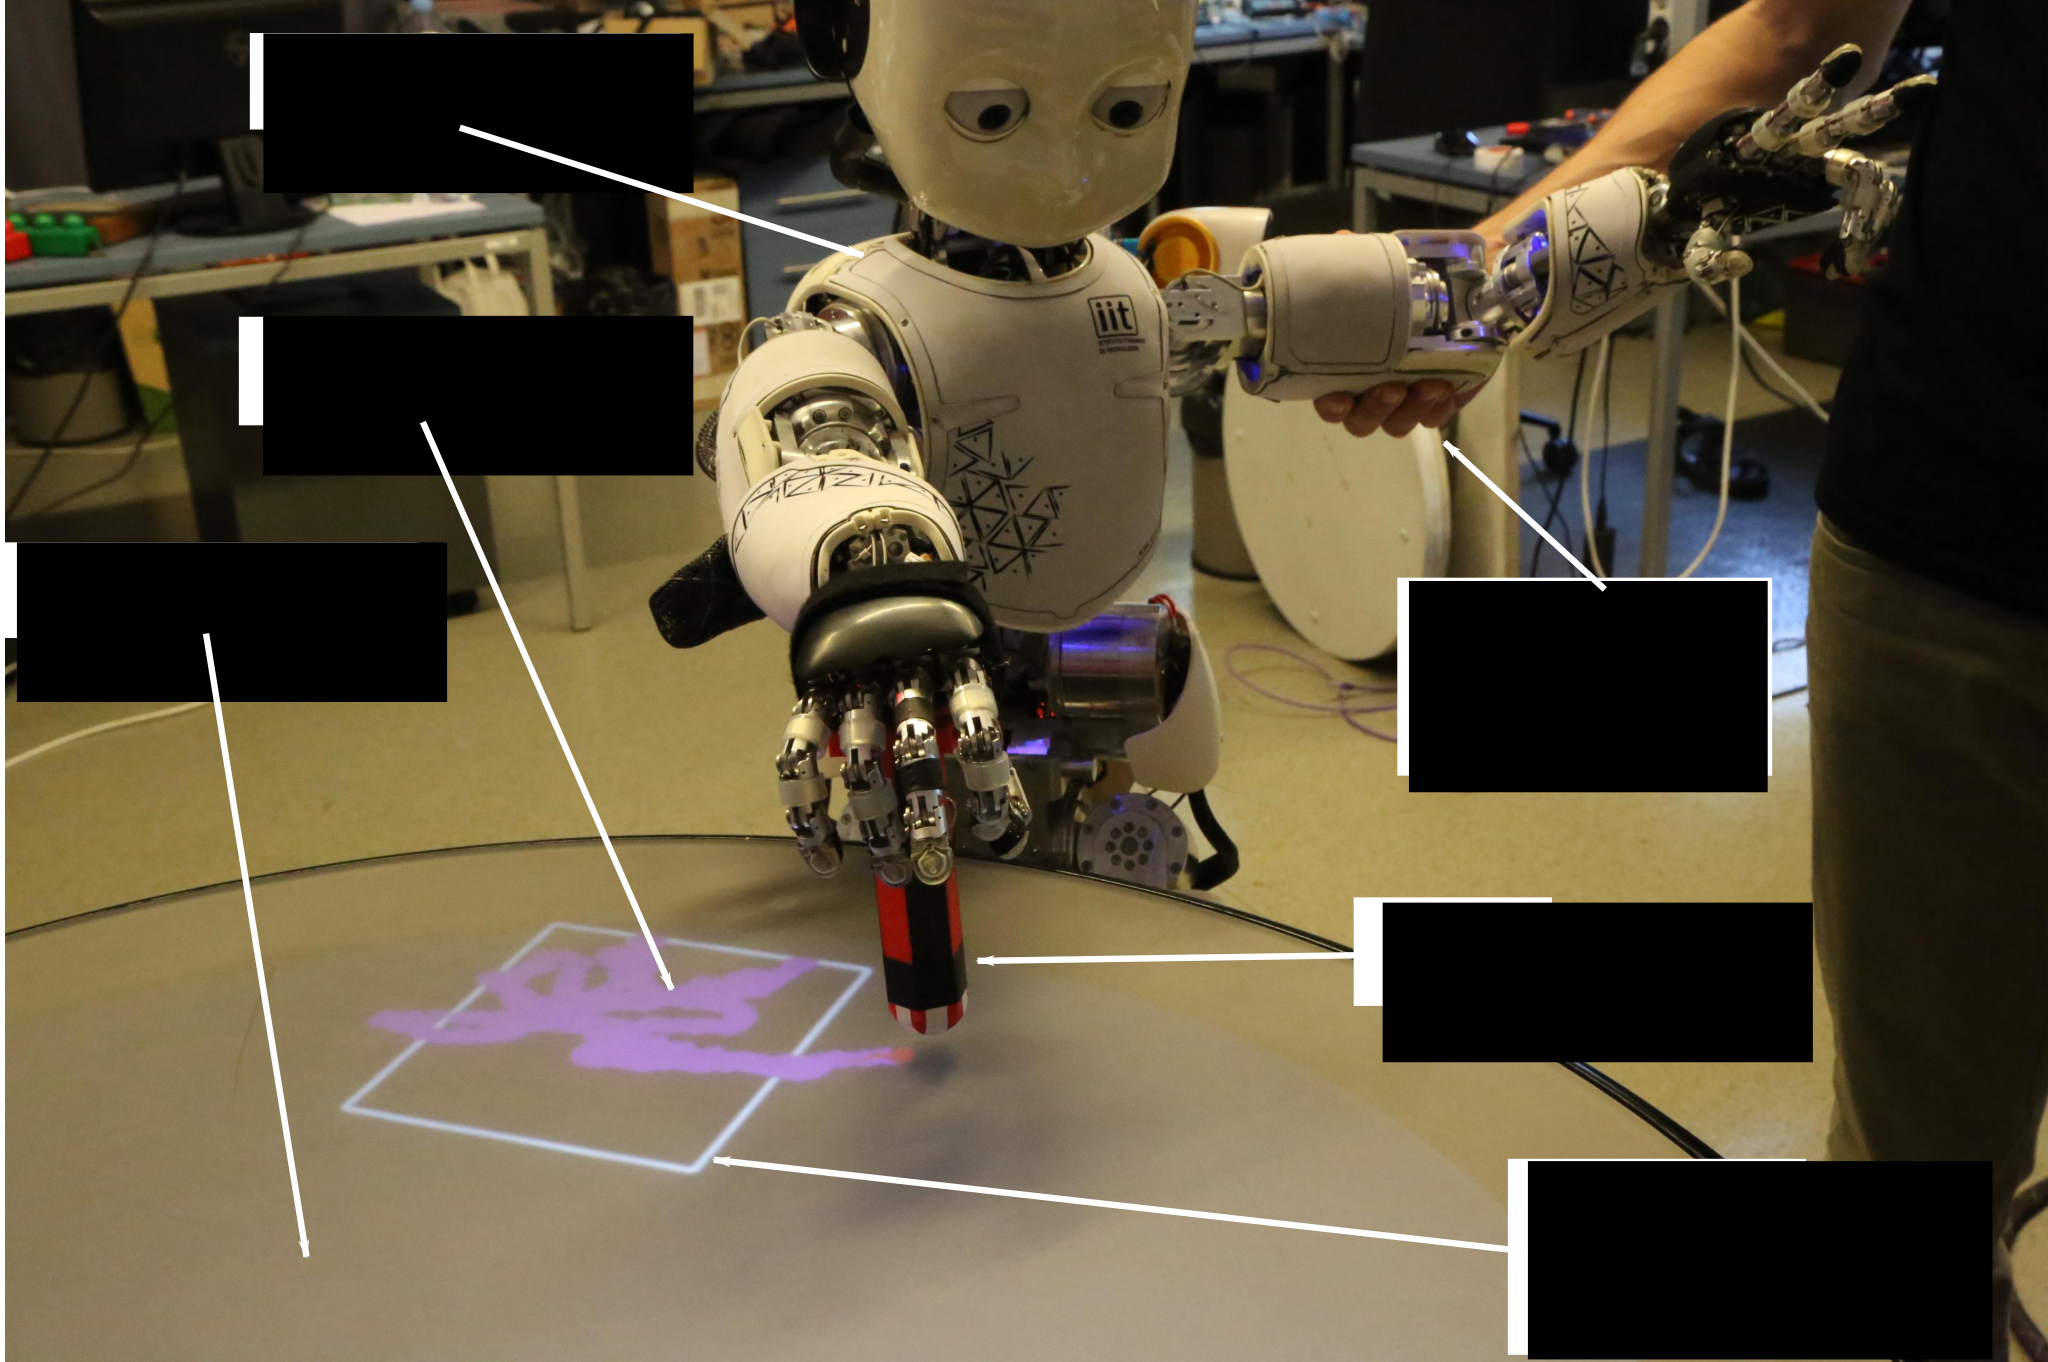
\includegraphics[width=8cm]{setup}
\caption{Our experimental setup consists in a humanoid iCub robot, a 3D-printed pen, and an interactive table called the Reactable.}
\label{fig:setup}
\end{figure}
\cmf{todo: Here a picture of the whole setup, with legend indicating the iCub with the tactile skin and working arm, the Reactable, the pen, the working area, the shape to be painted}

 
The neuro-controller we are going to describe outputs $(x, y)$ coordinates inside the working area that the robot can reach by moving its whole body as instructed by the inverse-kinematics module. It consists in two coupled control loops: a reactive and an adaptive ones.

\subsection{Reactive Controller}

The reactive controller provides the robot with two needs. The first one corresponds to a basic exploratory behavior which drives the robot to move the pen in random directions. A direction is defined by a random angle sampled uniformly in $[0, 2\pi]$ and a random distance  sampled from a normal distribution with mean \cmf{to fill} and standard deviation \cmf{to fill}. The second need is a reactive behavior which drives the robot hand to the starting position. This behavior is triggered by an input $h \in [0,1]$ to the reactive controller, such that the robot's hand moves to the center with a distance proportional to $h$, i.e. completely to the center when $h=1$ and at equidistance of the current hand position and the center when $h=0.5$. The safety behavior is only triggered when $h$ is above a small threshold $\epsilon$, otherwise the exploratory behavior operates in isolation. 

At the reactive level, the safety behavior is triggered from the perception of a strong grasp on the robot's left arm, which activates the reactive controller input with $h=1$. In the terms of the biological background of section \ref{{sec:reactive_bio}, the grasping perception can be viewed as the crossing of the comfort zone boundary and the safety behavior as the reactive action supposed to bring the homeostatic variable back into the CZ.  This way, the robot performs random drawing when the pen is inside the shape and each time its goes outside of it, the human subject grasps the robot's left arm, which triggers in turn the safety behavior returning in the center of the working area.

\subsection{Adaptive Controller}

The adaptive controller learns to anticipate the tactile feedback based on the perception of the distance between the pen tip and the closest shape boundary. For this it simply acts as a linear regressor whose target signal is the negative reinforcement provided by the human. As bases of this approximation it uses a repertoire of time-varying signals that code contextual information, the analogue of CS in classical conditioning, which in this setup is provided by the distance between the pen and the closest boundary. 

The generation of this context-coding signal comprises two steps. First $n$ \ih{to jordi: how many?} bases output a $1$ when the distance \ih{in pixels?} to the boundary is less than a given threshold value and $0$ otherwise, where each basis has a different threshold. This can then be interpreted as the controller receiving a set of CSs. Once these signals enter the adaptive controller, they are replicated n-times and passed through a series of double-convolutional filters with different temporal profiles (the details can be found in \ref{herreros2013speed}) to generate a series of diverse time-varying signals. We refer to these signals as \emph{cortical bases}. At time $t$, the vector $\mathbf{p}(t)$ contains the state of these bases. The output of the adaptive controller, that by analogy with the conditioning paradigm we refer to as $CR$ is equal to $\mathbf{p}(t)^T \mathbf{w}(t)$, where $\mathbf{w}(t)$ are the regression weights.

The controller regresses its teaching signal $e(t)$ to the context at time $t-\delta$. The regression weights $\mathbf{w}(t)$ are learned on-line using the decorrelation learning rule \cite{fujita1982adaptive}:

\[
\dot{\mathbf{w}}(t) = -\eta \mathbf{p}(t-\delta) e(t)
\]

where $\eta$ is a sufficiently small learning rate. Finally, the error signal is computed as follows

\[
e(t) = US(t) - k_{noi} CR(t-\delta)
\]

This implies that the adaptive controller requires a degree of feedback to confirm the correctness of the anticipatory action, otherwise a negative error would be generated, proportional to the $k_{noi}$ factor, resulting in the extinction of the acquired behavior. In our setup, since the feedback is binary, this will lead to a non-zero error rate at learning asymptote. Note that the human reinforcement is compared not to the current output of the controller but to a preceding one at time $t-\delta$, denoting that if an error occurs at time $t$ it should have been prevented not by an action simultaneous to the error, but by one anticipated by $\delta$ seconds. In short, this $\delta$ sets the extent of the anticipation.

\begin{figure}[!t]
\centering
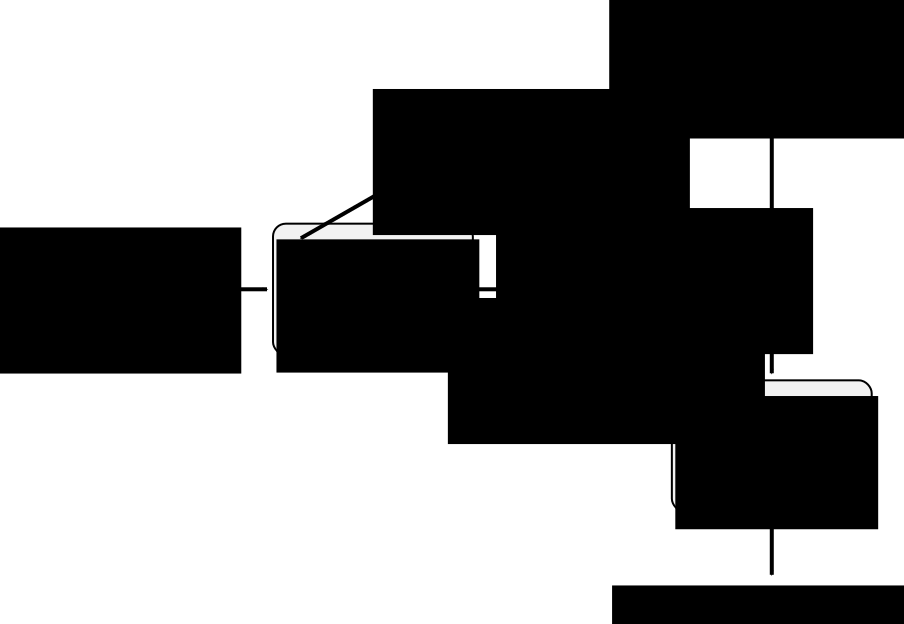
\includegraphics[width=8cm]{architecture}
\caption{.}
\label{fig:architecture}
\end{figure}

%\subsection{Tying Everything Together}
%In this article we present the combined model of using self-regulation or homeostasis as the generator of the signal that must be anticipated by the cerebellum. In this combination, we chose to use high level needs so that we can generalize 



\section{Results}
\label{sec:results}

We instructed a human subjects to grasp the robot's upper left arm every time the pencil crossed the boundary of the shape, and release it after it entered back. For the first round of experiments, the shape was always a square. The subject was presented 10 times with the reactive controller and 10 with the adaptive controller on top of it. 
Figure \ref{reactive} shows a sample of both conditions. One can observe increases in both, the number of times the robot received feedback and the amount of time spent on average with every feedback for the reactive condition with respect to the adaptive. \jp{Generate numbers!}. Comparing figures \ref{reactive} B and D show how

We instructed a human subject ...
with details but not too much

Figure x shows ...


\begin{figure*}[bc]
\centering
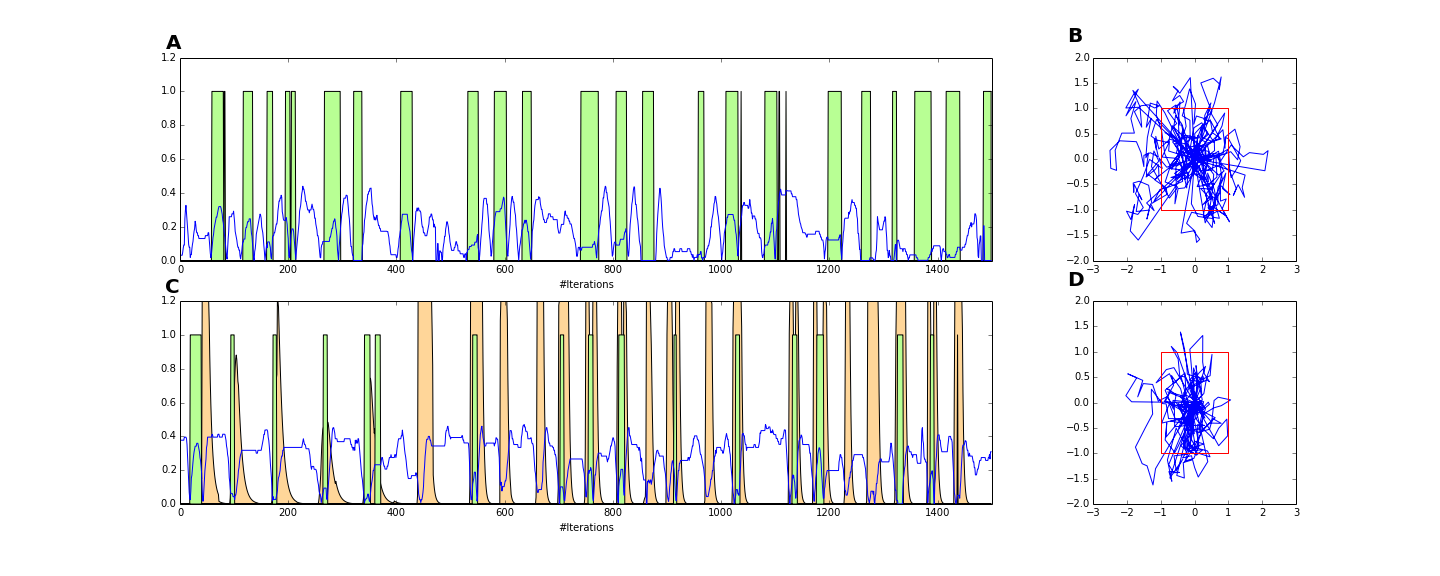
\includegraphics[width=20cm]{reactive_adaptive}
\caption{This figure shows a comparison of the reactive (A,B) and the adaptive (C,D) behaviors. On A and C, the blue line shows the \emph{cs} as detailed in equation \ref{cs}. Green stripes show human feedback (US) as unit steps for the duration of the contact. For the adaptive behaviour, orange shows the cerebellum output. From iteration 250, anticipation of human feedback can be observed. Figures B and D show the behavior of the pencil on the table. \jp{check that this is true, after all!}}
\label{fig:reactive}
\end{figure*}




\begin{figure}
\centering
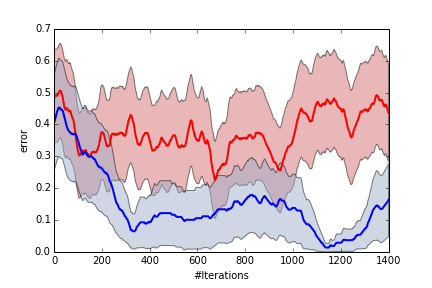
\includegraphics[width=9cm]{error}
\caption{The experiment was realized 10 times, initializing all the parameters. This figure shows the mean (red) and standard error (grey) of the time that robot had human feedback. Dashed lines show the results of each experiment. }
\label{fig:error}
\end{figure}

\section{Discussion}

Being the error nonspecific, in the sense that it only signals the aversive state but it does not contain information about how to correct it, one could argue that a Reinforcement Learning (RL) paradigm would have been more adequate; but we justify in the following why this is not the case. Our problem here is to generate rapid anticipatory well-timed responses, which is precisely the role of a cerebellar like structure.

The used cerebellar model \cite{herreros2013nucleo} is a supervised learning system that in our case is driven by a nonspecific error from human feedback. The trick is that learning is anticipating the triggering of the reactive behaviour in advance which in itself contains information on the movement to make. Although the error is nonspecific, the contextual information needed for the reflexive action to generate the appropriate reflex directed to the center of the shape is contained in the reactive layer. Our aim is to model using a complete developmental scenario, how the cerebellum is involved in adaptively modulating reflexive behaviour. Moreover with the cerebellar architecture, we get generalisation to different execution speeds for free since the first trials \cite{herreros2013speed}.  

In the future we will consider of making the human feedback more specific, by for example being able to translate a tactile pattern, while holding the forearm of the iCub, into a correcting direction. We could consider as well using the force feedback sensing of the iCub for this purpose.


\section{CONCLUSIONS}
\label{sec:conclusions}

...

It is clear that this system will fail to anticipate when contextual cues are noisy or imprecise. For this reason, we propose the use a two phase model of learning [reference] that, independently from the prediction phase, uses the US [CHECK THAT US HAS BEEN DEFINED BEFORE] to learn to effectively represent significant stimuli (good or bad). This perceptual phase is grounded on the observed increase in plasticity in the sensory cortex in presence aversive or rewarding stimuli. This model should then be able to learn the relevant perceptual blocks that allow a consistent and robust anticipation of reward or punishment. 

...

\addtolength{\textheight}{-12cm}   % This command serves to balance the column lengths
                                  % on the last page of the document manually. It shortens
                                  % the textheight of the last page by a suitable amount.
                                  % This command does not take effect until the next page
                                  % so it should come on the page before the last. Make
                                  % sure that you do not shorten the textheight too much.

%%%%%%%%%%%%%%%%%%%%%%%%%%%%%%%%%%%%%%%%%%%%%%%%%%%%%%%%%%%%%%%%%%%%%%%%%%%%%%%%
\begin{comment}
\section{EUCOG abstract}
We present a model of the control of hand movements learned from human feedback. The setup consists in an iCub humanoid robot able to paint with its finger tip on an interactive display, the Reactable. It learns how to paint inside a closed shape, e.g. a circle, which is drawn on the table and from which the robot can perceive the boundaries. Before learning, the robot does not know that it has to paint only inside the boundaries. This is instead learned from negative human feedback provided whenever the robot’s finger tip goes outside of the shape, using a neurocomputational model of the cerebellum learning how to anticipate the negative feedback from the perception of the shape boundaries. 

Our model consists in a reactive and an adaptive controllers. The reactive controller defines two needs of the robot. The first one drives the robot to move the virtual pen on the table in random directions, without taking into account the perception of the shape boundaries. The second need drives the robot to move the pen in the opposite direction whenever it perceives a negative human feedback. We show that this simple reactive controller, when acting in isolation, allows to roughly paint inside the shape although it often crosses the shape boundaries as an untrained young infant would do.

On top of this purely reactive system, an adaptive controller tries to make sense of the human feedback to optimize behavior, i.e to minimize the amount of negative feedback it will receive -- and consequently to paint with more precision. The adaptive controller aims at learning how to perform anticipatory actions to avoid the human negative feedback. It is based on a neurocomputational model of the cerebellum which functionally acts as a function approximator and learns to predict the negative feedback from the perception of the shape boundaries relatively to the position of the finger tip. Because the human feedback is correlated with the distance between the finger tip and the closest shape edge, the adaptive controller learns to perform the compensatory action, i.e. the moving of the finger tip in the opposite direction, whenever the latter becomes too close from a shape boundary. 

We show how this biologically-inspired adaptive mechanism, which is plausible in terms of human infant development, allows the learning of a precise painting behavior, using the perception of the shape boundaries as a predictive signal of negative feedback. This mechanism can be generalized to any kind of task where negative feedback can be predicted by sensory cues.

\end{comment}

%%%%%%%%%%%%%%%%%%%%%%%%%%%%%%%%%%%%%%%%%%%%%%%%%%%%%%%%%%%%%%%%%%%%%%%%%%%%%%%%



%%%%%%%%%%%%%%%%%%%%%%%%%%%%%%%%%%%%%%%%%%%%%%%%%%%%%%%%%%%%%%%%%%%%%%%%%%%%%%%%
\section*{APPENDIX}

Appendixes should appear before the acknowledgment.

\section*{ACKNOWLEDGMENT}

The preferred spelling of the word ÒacknowledgmentÓ in America is without an ÒeÓ after the ÒgÓ. Avoid the stilted expression, ÒOne of us (R. B. G.) thanks . . .Ó  Instead, try ÒR. B. G. thanksÓ. Put sponsor acknowledgments in the unnumbered footnote on the first page.



%%%%%%%%%%%%%%%%%%%%%%%%%%%%%%%%%%%%%%%%%%%%%%%%%%%%%%%%%%%%%%%%%%%%%%%%%%%%%%%%

\bibliographystyle{IEEEtran}
\bibliography{humanoids}





\end{document}